\documentclass[12pt,openright,oneside,a4paper,brazil]{abntex2}
\usepackage[utf8]{inputenc}
\usepackage[T1]{fontenc}
\usepackage{graphicx}
\usepackage{listing}
\usepackage{amsfonts}

\title{Projeto Interativo III - Angry Robots}
\date{}
\author{\textbf{Caroline Bomfim Do Espirito Santo} (caroline.bomfim@hotmail.com.br), \\ \textbf{Mahaira Soares de Souza} (mahaira\_souza@hotmail.com), \\ \textbf{Rafael da Silva Santos} (rafa\_silva.santos@hotmail.com), \\ \textbf{Thiago de Sousa Messias} (messiasthi@gmail.com). \\ \\ Ciência da Computação - Centro Universitário Senac}

\setlength{\parskip}{0.2cm} 
\setlrmarginsandblock{3cm}{2cm}{*}
\setulmarginsandblock{3cm}{2cm}{*}
\checkandfixthelayout

\begin{document}

\maketitle
 
\section*{Resumo}

Angry Robots é um jogo desenvolvido em linguagem C, utilizando a biblioteca gráfica allegro 5, fundamentado em visão computacional aplicando inderetamente o "OpenCV". Um de seus principais objetivos é induzir o usuário a trabalhar sua mente e desenvolver seu racíocinio lógico, com estratégia e agilidade para derrotar o robô. A parte de visão computacional foi construida com algotitmos em função do cálculo da centróide e o sistema de cores HSV (formado pelas componentes Hue (tonalidade), Saturation (saturação) e Value (valor).

\textbf{Palavras-chave:} algoritimo, OpenCV, allegro, biblioteca gráfica, HSV.

\section*{Abstract}

\textit{Angry Robots is a game developed in C language, using the graphics library allegro 5, based on computer vision indirectly applying the "OpenCV". One of its main objectives is to induce the user to work your mind and develop your logical thinking with strategy and agility to defeat the robot. Part of computer vision was built with algorithms depending on the calculation of the centroid and the HSV color system.} \\

\textbf{Keywords:}\textit{ algorithm, OpenCV, allegro, graphics library, HSV.} 

\section*{Introdução}

Nos últimos anos a industria de jogos cresceu de forma constante, e com ela a importância dos mesmos para o desenvolvimento de muitas habilidades humanas. Sabemos que a maioria dos jogos são desenvolvidos com intuito de estabelecer uma conexão entre o mundo virtual e o real, para que desta forma possa proporcionar ao jogador tanto uma diversão quanto o desenvolvimento de suas habilidade pessoais, como agilidades, raciocínio lógico, estratégia, entre outros, assim lhe ocasionando um exercício mental. \\
Angry Robots, faz com que o jogador se movimente de forma rápida e lógica para que consiga chegar ao objetivo final, ganhar a partida e derrotar o robô. \\
Em relação a visão computacional, quando tratada a imagem, utiliza-se algorítimos e fórmulas matemáticas, e principalmente a física, fundamental para calcular a frequência e tonalidade de cores, a iluminação e luminosidade do local, de maneira que possamos descobrir em qual escala de cor se encontra e melhorar a qualidade visual do jogo.

\section*{Revisão de Literatura}

Angry Robots é um jogo limitado, pois dentro das exigências foram permitidos somente as bibliotecas, allegro 5 graficamente e a multiplataforma OpenCV utilizada para desenvolvimento de aplicativos na área de visão computacional. \\
Existem diversos jogos em que o Angry Robots foi baseado, um deles foi o Cube Slam, um jogo em que os usuários se enfrentam numa partida visual de air hockey, no qual o jogador luta contra um urso, já no Angry Robots o adversário é um robô rápido e ágil. \\
Há projetos no blog "Laboratório Garagem", entretanto todos fugiam do ambiente proposto, a maioria deles utilizavam Arduíno, OpenCV e Python. Porém, mesmo com os obstáculos impostos no Angry Robots, foi de grande utilidade pois algumas ideias surgiram através de post's referentes à robôs. \\
Gran Slam Tennis 2, jogo que simula os grandes campeonatos de tênis, foi utilizado como base para os movimentos do jogo. \\ 
Os algorítimos desenvolvidos são autorais sem base em outros jogos, visto que mesmo com fundamento em tantos jogos, Angry Robots é um diferencial.

\section*{Desenvolvimento}

\textbf{Histograma}:
Um histograma, conhecido também como distribuição de frequências. Aplicado no código para captar os tons de azul, onde todos os valores abaixo da media automaticamente serão zerados e os maiores maximizados, para que se encaixem no tom rastreado, calculando assim o centro.
\\ \\ \\ \textbf{Centróide}:
É o ponto interior que define seu centro geométrico, caso a forma geométrica represente uma secção homogênea de um corpo, então o centroide coincide com o centro de massa. A mesma foi implementada no Angry Robots para captar o meio da tela, facilitando a detecção e visualização do restante do display para uma variação é identificação da cor de preferência, no caso o azul. 
\\ \\ \textbf{Conversão para HSV}: 
Calcula a intensidade da tonalidade, saturação e brilho da imagem, possibilitando aprimoramento no rastreamento do código, para resolver problemas com a iluminação do local, assim, não atrapalha a jogabilidade. A tonalidade permite distinguir as cores puras de 0 á 360 graus, a saturação verifica a intensidade da pureza da tonalidade, o brilho verifica a iluminação da imagem. 

\begin{figure}[!htb]
\centering
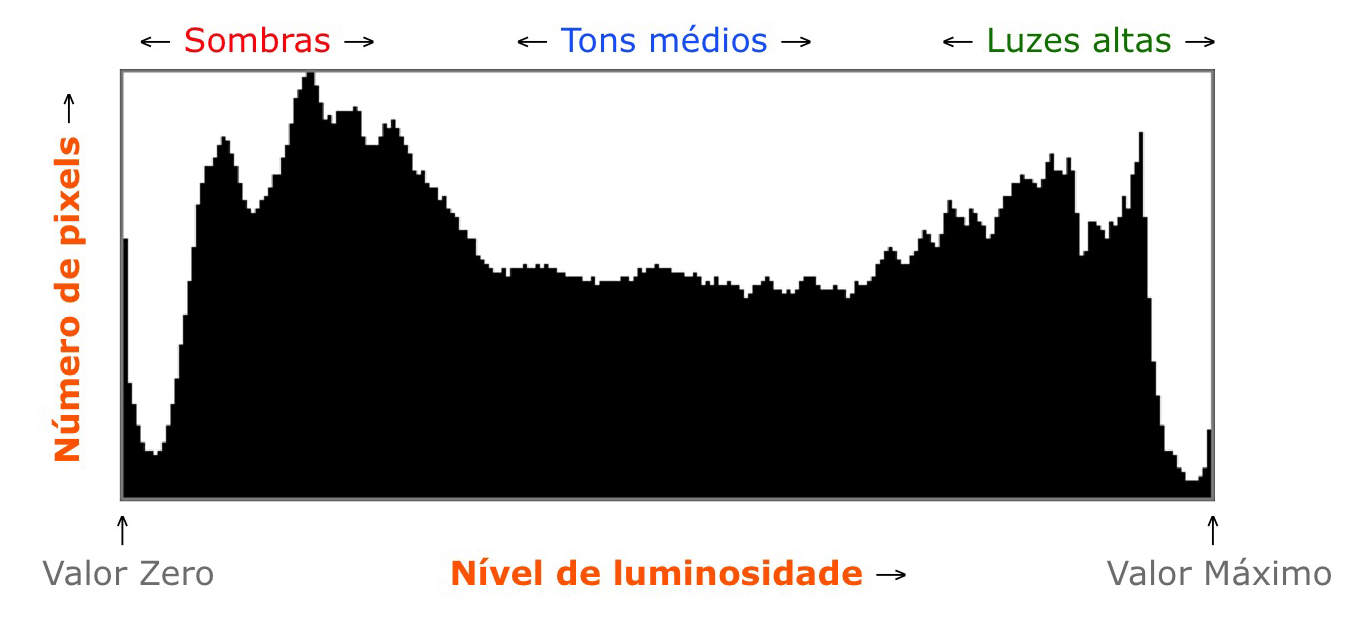
\includegraphics[scale=0.2]{histograma.jpg}
\caption{Exemplo: Nivél de frequência da cor.}
\end{figure}

\section*{Resultados}

Neste jogo o robô ira tentar fugir para que o jogador não consiga acerta-lo com pequenas bolas, 
isto será feito através de um laser azul, o objetivo do jogo é derrotar o robô jogando as bolas em sua direção, quanto mais rápido os movimentos do usuário, mais chances de vencer o jogo.

\begin{figure}[!htb]
\centering
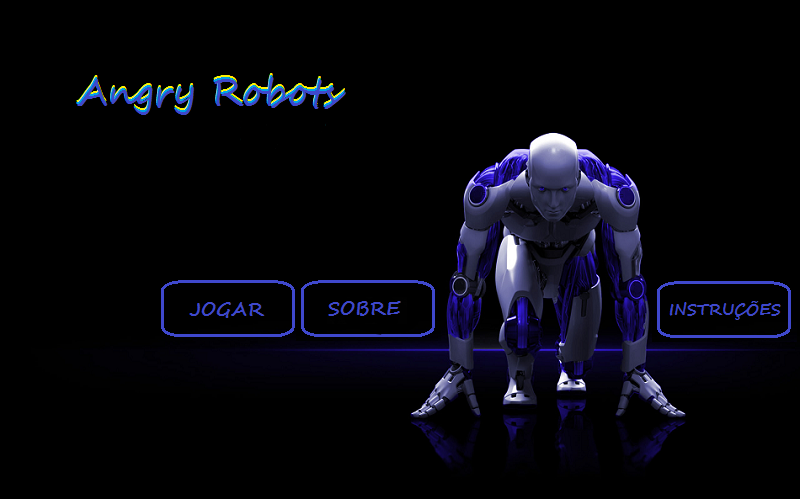
\includegraphics[scale=0.3]{menu.png}
\caption{Imagem do jogo funcionando}
\end{figure}
\vspace{0.5cm}

\begin{figure}[!htb]
\centering

\includegraphics[scale=0.3]{fundo.jpg}
\caption{Imagem do jogo funcionando}
\end{figure}
\vspace{0.5cm}

\section*{Considerações Finais}

O rastreamento é o ponto mais difícil, pois alguns fatores atrapalharam o desenvolvimento do mesmo, um deles foi a iluminação, pois devido a ela, a imagem pode ser ofuscada ou obscurecida demais, porém o HSV permitiu que a iluminação fosse ignorada, pois este algoritmo converte toda a imagem para cinza, e trata a variação da luminosidade, deste modo o usuário poderá jogar com uma camiseta azul por exemplo, sem afetar o rastreamento.

\begin{thebibliography}{6}
\bibitem *http://labdegaragem.com/profiles/blog/list?tag=rob\%C3\%B3tica \\
\bibitem *http://labdegaragem.com/profiles/blog/list?tag=rob\%C3\%B4 \\
\bibitem *http://www.techtudo.com.br/noticias/noticia/2012/02/top-10-jogos-com-robos-gigantes.html \\
\bibitem *http://www.di.ubi.pt/~agomes/cg/teoricas/06-iluminacao.pdf \\
\bibitem *http://sidigicor.blogspot.com.br/2011/02/modelo-hsv.html \\
\bibitem *http://www.ufrgs.br/engcart/PDASR/formcor.html

\end{thebibliography}

\end{document}